The top quark induced background in the \WW\ analysis originates from
\ttbar\ and the single top (\tw) processes, the latter being especially imporatant 
in the 0-Jet bin.  A consistent theoretical description of the two
processes at high perturbation orders is not straightforward to attain
as already at NLO some \tw\ diagrams coincides with LO \ttbar\
ones \cite{singleTopInterference}.  The Monte Carlo simulated samples
used in the analysis exploit an approach recently
proposed \cite{singleTopRemoval}, which addresses the overlap by
discarding the common diagrams from the \tw\ process either at
amplitude level ({\it Diagram Removal}) or at cross section level
({\it Diagram Subtraction}).  The former is considered the default
scheme, whereas the latter is used as cross check.

The top background is estimated at the \WW\ preselections level where
a common scale factor for the Monte Carlo \ttbar\ and \tw\ samples is
computed.  Once properly normalized, those samples are used either to
predict the correspoding yields after the mass dependent Higgs
selections for the cut based analysis (Section \ref{sec:anal_cutbased}), 
or as templates for the multivariate analysis.

The procedure for top background estimation can be summarized as follows.
The top background is suppressed using top tagging veto (Section~\ref{sec:sel_toptag});
if the tagging efficiency is known, the top background can be estimated using the formula:
\begin{equation}
N_{top-veto} = N_{top-tag} \times (1-\epsilon_{tag})/\epsilon_{tag},
\end{equation}
where $N_{top-veto}$ is the number of top events that pass the veto, $N_{top-tag}$ is the 
number of top events that are top-tagged and $\epsilon_{tag}$ is the top tagging efficiency
as measured in a control region dominated by top events.
Both in the evaluation of $N_{top-tag}$ and $\epsilon_{tag}$, non-top backgrounds are properly 
subtracted using data-driven or MC estimates depending on the process.
The systematic uncertainty on the top estimation is due to the uncertainty on non-top 
backgrounds and on the statistical error in the efficiency measurement.
The actual implementaion of the estimation method depends on the jet bin.

% %%%%%
% \begin{table}[!h]
% \begin{center}
% \begin{tabular} {|c|c|c|c|c|}
% \hline
% jet bin & top veto & top tag & $\epsilon_{tag}$ denominator & $\epsilon_{tag}$ numerator \\ 
% \hline
% 0       & no soft muon,      & either a soft muon  & 1-jet bin, leading & denom. + \\
%         & no low \pt\ b-jets & or a low \pt\ b-jet & jet is btagged     & top tag  \\
% \hline
% 1       & no soft muon,           & leading jet  & 2-jet bin, sub-leading & denom. + \\
%         & no low/high \pt\ b-jets & is b-tagged  & jet is btagged         & top tag  \\
% \hline
% 2       & no soft muon,           & central jet  & 2-jet bin, no & denom. + \\
%         & no low/high \pt\ b-jets & is b-tagged  & VBF selection & top tag  \\
% \hline
% \end{tabular}
% \caption{Summary of selection and control region definitions used in top estimation in the different jet bin.}
% \label{tab:topbkgest}
% \end{center}
% \end{table}
% %%%%%

%
% ZERO JET BIN
%
\subsubsection{0-Jet Bin Method}

The procedure to estimate the top background from data in the case of
the 0-Jet bin established in \cite{HWW2011} has been adapted to the
most recent theoretical description of \ttbar\ and \tw{} in \cite{HWWFull2011}.
The latter is used in the present analysis and briefly described here.

Rejection for the top background is achieved by top-tagged events,
i.e. events with a b-tagged jet or a soft muon as defined in
Section~\ref{sec:sel_toptag}.  The estimation of this background
relies on the measurement on data of the top-tagging efficiency.  

In the 0-jet bin, the key ingredient for top estimation, is that \ttbar\ events 
are carachterized by two b-jets below 30 GeV, while \tw\ events have one 
single low \pt\ b-jet except for a fraction $x$ containing two jets from 
b quarks and effectively indistinguishable from \ttbar.
The procedure described in the following steps accounts for this feature properly:

\begin{itemize}

\item 
A top enriched region is defined requiring exactly one b-tagged jet
with \pt\ larger than $30$ GeV (denominator).  Those events among this
sample with at least one b-tagged jets with
$10<\ensuremath{p_\mathrm{T}}<30$ GeV or one soft muon defines the
numerator. The ratio of the yields in the numerator and denumerator
provides the top-tagging efficiency for one ``top-taggable'' leg,
$\epsilon_{1leg}^{data}$.
This efficiency is computed for \ttbar\ only, i.e. non-top 
backgrounds and \tw\ yields are subtracted from the measured data in 
the control region (both numerator and denominator).  
The yields for \tw\ are estimated from the Monte Carlo normalized accordingly to
the data-driven predictions in the 1-Jet bin previously evaluated.

\item 
The overall top-tagging efficiency, $\epsilon_{topTag}^{data}$, is
defined to account for the fraction of \tw\ events that looks
like \ttbar\ ($x$), that is with two top-taggable legs:
\begin{equation} \label{eq:newTopTagEff}
\epsilon_{topTag}^{data} = (f_{t\bar{t}}^{MC} + x(1-f_{t\bar{t}}^{MC}) )(1-(1-\epsilon_{1leg}^{data})^2) + (1-f_{t\bar{t}}^{MC})(1-x)\epsilon_{1leg}^{data}
\end{equation} 
where the first term on the right accounts for events with two taggable
legs and the second term for one taggable leg. 
$f_{t\bar{t}}^{MC}$ represents the fraction of \ttbar\ events with respect to the total \ttbar+\tw\ 
and it is determined from Monte Carlo in the 0-Jet bin at the \WW\ preselection level, removing the anti top-tagging.
The fraction $x$ matches the value of $\epsilon_{1leg}$ estimated from
the \tw\ Monte Carlo.  We consider this a good approximation as
$\epsilon_{1leg}$ is the fraction of events with one b-tagged jet
with \pt larger than 30 GeV (the first ``top-taggable'' leg) and
top-tagged leg (a b-tagged jets below 30 GeV or a soft muon).

\item 
A dedicated control region is defined in the 0-Jet bin by requiring
top-tagged events.  The data yields in this region corrected for the
other backgrounds contaminations are then used together with
top-tagging efficiency to predict the top background after \WW\
preselections level:
\begin{equation} \label{eq:topExtrapolation}
N^{top}_{WW region}=N_{topTag}^{top}\frac{1-\epsilon_{topTag}^{data}}{\epsilon_{topTag}^{data}} = 
(N_{topTag}^{data}-N_{other-bkg}^{data})\frac{1-\epsilon_{topTag}^{data}}{\epsilon_{topTag}^{data}}
\end{equation} 

\end{itemize}

%
% ONE JET BIN
%
\subsubsection{1-Jet Bin Method}
To measure the tagging efficiency in the 1-jet bin we use top events 
with two reconstructed jets as the control sample. 
The expected tagging efficiency in simulated $t\bar{t}$ events after the $WW$ preselection
is shown using all jets and soft-muons and for the highest $\pt$ jet only
as a function of the number of counted jets in Figure~\ref{fig:btag_njets_highestptjet}.
The tagging efficiency for the highest $\pt$ jet is approximately
the same for the 1-jet and 2-jet bins. Therefore, we use the 
tagging on the highest $\pt$ jet and measure its efficiency in
the 2-jet bin where, in order to increase the top purity, 
the second jet is required to be b-tagged.

\begin{figure}[!htbp]
\begin{center}
% 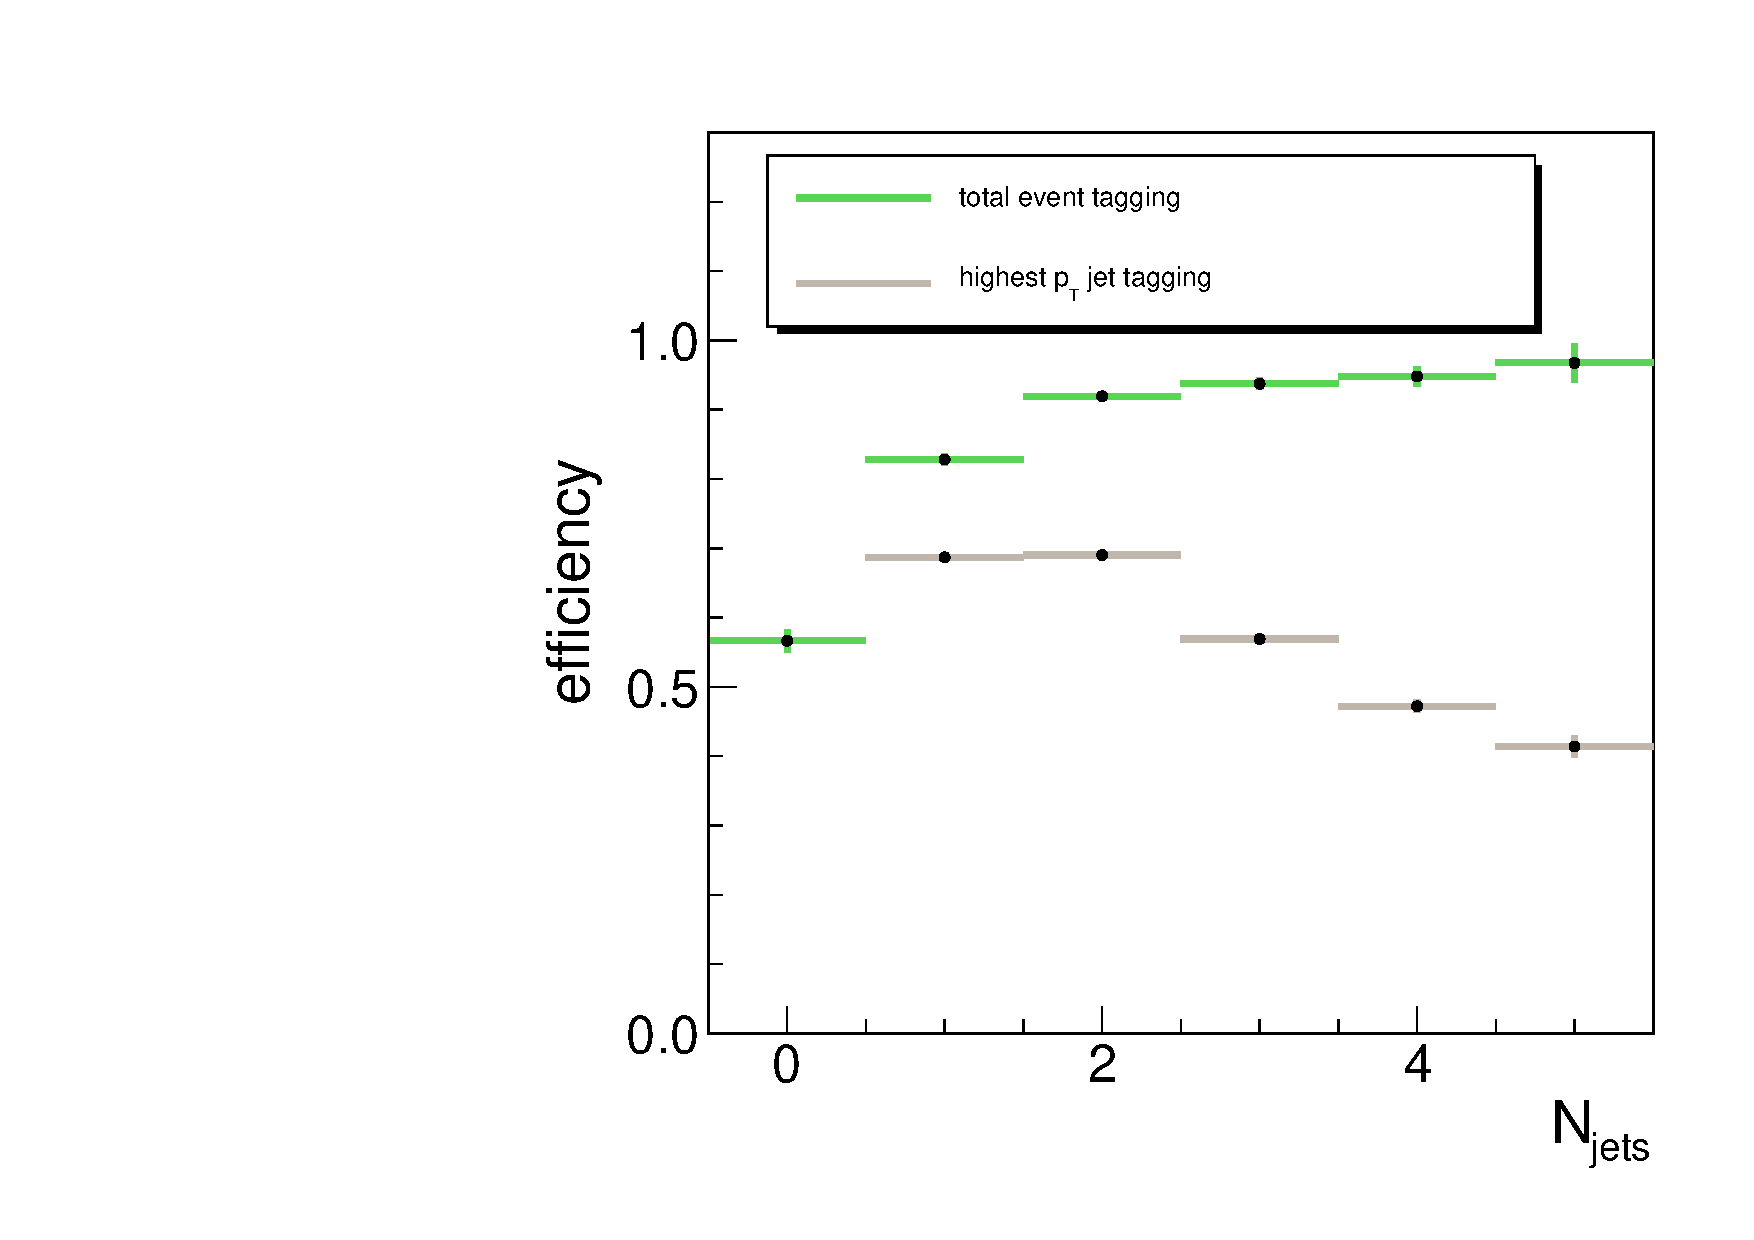
\includegraphics[width=0.55\textwidth]{figures/btag_njets_highestptjet.pdf}
\caption{\fixme Total tagging efficiency and tagging efficiency for the highest
$\pt$ jet for simulated top events as a function of the number of reconstructed
jets in top events after applying the $\WW$-like selection.}
\label{fig:btag_njets_highestptjet}
\end{center}
\end{figure}

The residual number of top events in the 1-jet bin is then given by,
$${N_{no~tagged}^{1-jet} = N_{tagged}^{1-jet} \times (1-\epsilon_{highest~\pt~jet})/\epsilon_{highest~\pt~jet}},$$
where $N_{tagged}^{1-jet}$ is the number of events where the counted jet is
tagged and none of the other non-counted jets are tagged, and $\epsilon_{highest~\pt~jet}$ is the 
tagging efficiency for the highest $p_{T}$ jet measured from the 2-jet bin.
The closure test, comparing the estimate using this procedure with 
the simulation, gives agreement to within $1\%$.

The scale factor is actually derived in a region that is slightly different from the signal region, 
but then it is consistently applied to the MC yield in the signal region.
The difference is due to soft muons. In the signal region, events with soft muons are always rejected.
In the 1-jet top estimation, instead, soft muons are allowed inside the leading jet; 
this is done consistently in the top veto region, in the top tag region and in the efficiency measurement.
The reason is that, when a soft muon is present in the jet, its b-tagging efficiency is slightly higher
soft muons and b-tagging are correlated. To avoid this correlation, we measure top without any requirement 
on soft muons close to the jet.

%
% VBF
% 
\subsubsection{2-Jet Bin Method}
Estimation of the top background in the 2-jet bin is complicated due to 
the additional requirements applied to the jets to
select $qqH$-like events. The tagging effiency for the selected jets 
after applying such selection is smaller than that in the inclusive 
2-jet bin sample, since the selection enhances events with forward 
jets, which have lower tagging efficiency.

The proposed method is to measure the tagging efficiency of the most central 
jet in the event as a function of its $\eta$ in an inclusive top 
enriched control sample, and then apply that rate to fully selected events 
where the most central jet is top tagged. In this way the 
possible kinematical differences between the control and signal regions 
are taken into account.

Therefore, the residual number of top events in the 2-jet bin after applying the full 
$qqH$-like is given by,
$${N_{non~tagged}^{qqH} = N_{tagged}^{qqH} \times (1-\epsilon_{central~jet})/\epsilon_{central~jet}},$$
where $N_{no~tagged/tagged}^{qqH}$ is the number non-tagged/tagged events using 
the most central jet, and $\epsilon_{central~jet}$ is the 
tagging efficiency as a function of $\eta$ of the jet. The comparison of the 
$|\eta|$ distribution of the most central jet in top events after applying the $qqH$-like selection between the simulation and 
the prediction using top-tagged events is shown in Figure~\ref{fig:vbf_btagprediction_jetmin}, where 
good agreement in shape and normalization is observed in the region $|\eta|<2.5$. A small correction 
of about 10\% in the yield must be included in the prediction to take into account the fraction 
of top events where the most central jet is outside the tracker acceptance.

\begin{figure}[!htbp]
\begin{center}
%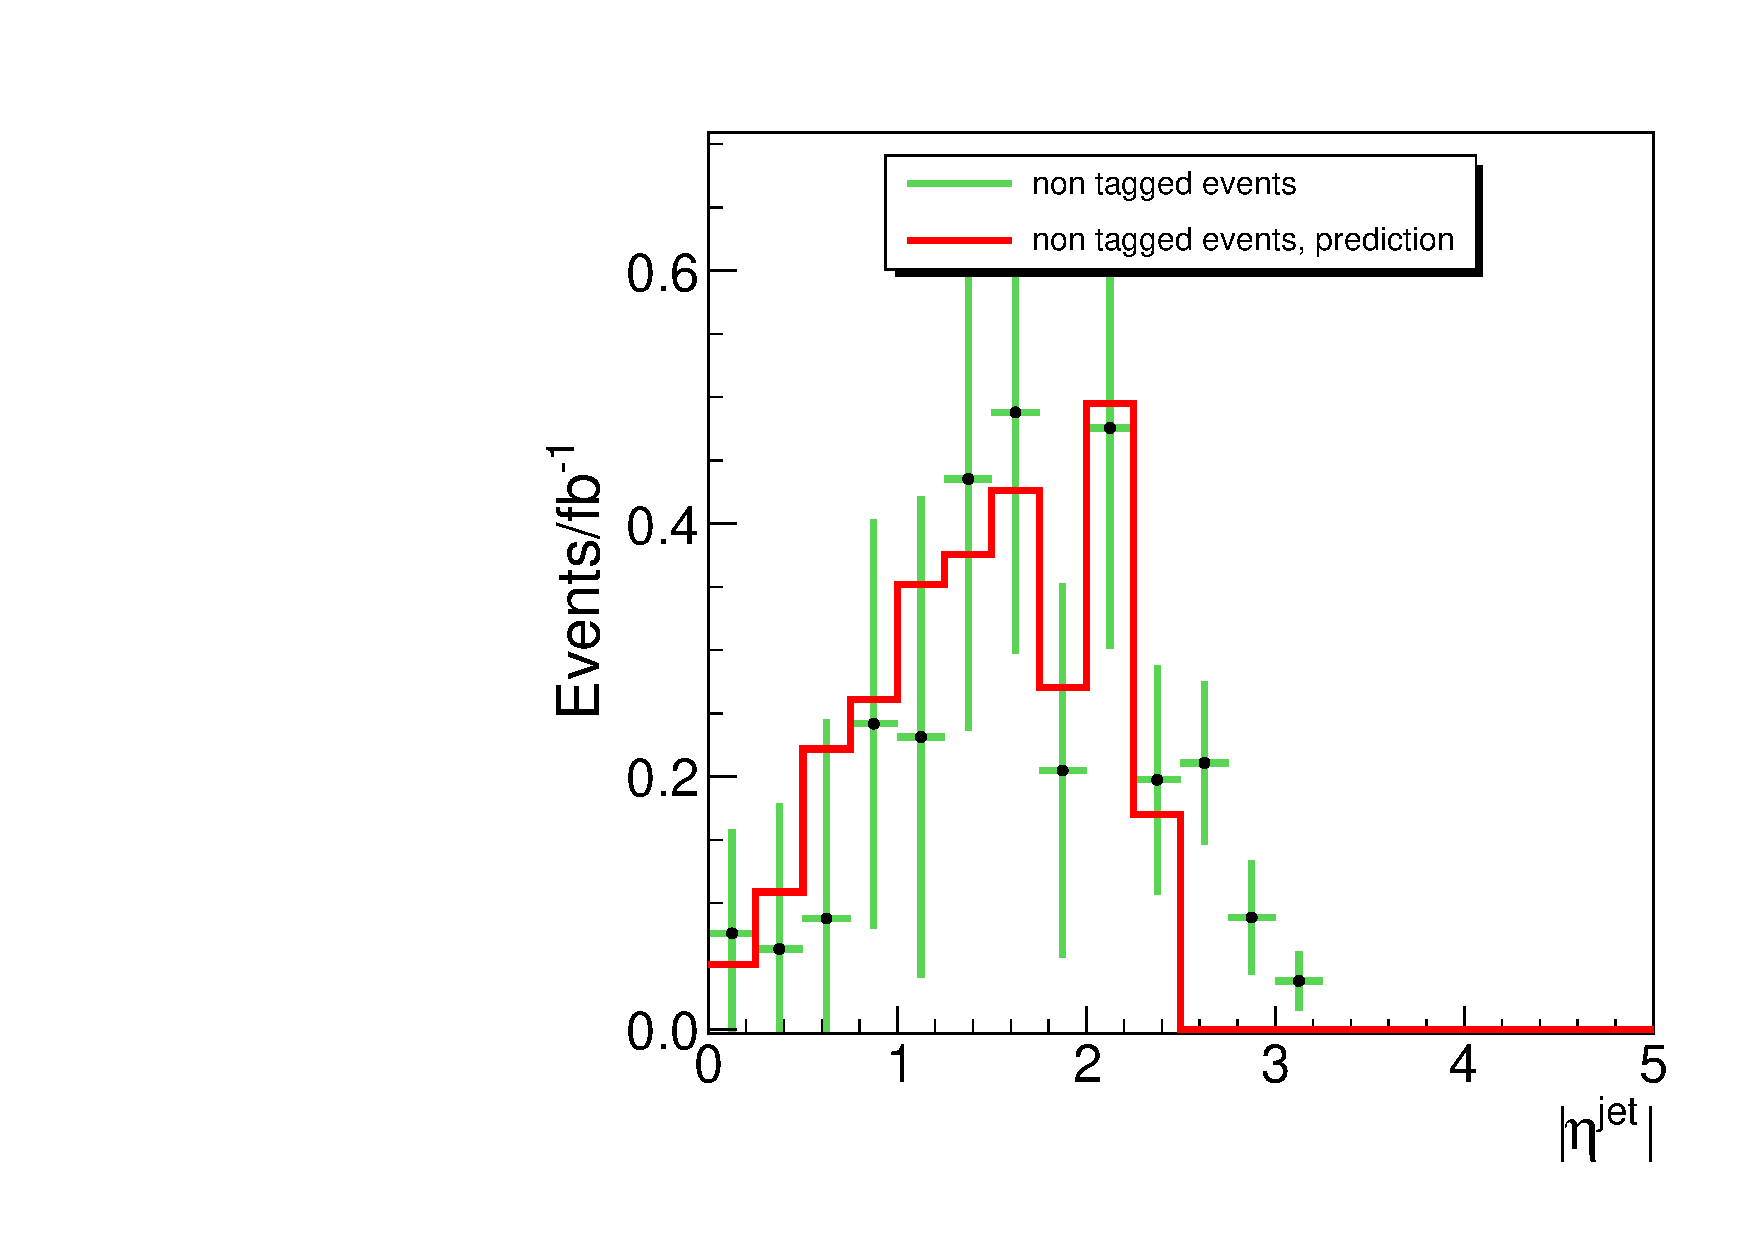
\includegraphics[width=0.65\textwidth]{figures/vbf_btagprediction_jetmin.pdf}
\caption{\fixme $|\eta|$ distribution of the most central jet in top events after 
applying the $qqH$-like selection. Comparison between the simulation and 
the prediction using top-tagged events.}
\label{fig:vbf_btagprediction_jetmin}
\end{center}
\end{figure}
